\subsubsection{Practices and Implementation} \label{sec:practices-implementation-weight}

%% PWF variables to fill in
\newcommand{\PWF}[0]{\mathcal{P}}
\newcommand{\minWeight}[0]{0.4}
\newcommand{\maxWeight}[0]{1.1}
\newcommand{\markForMinWeight}[0]{0.2}
\newcommand{\markForMaxWeight}[0]{0.825}
\newcommand{\markForUnity}[0]{0.597}

$\codebaseGrade$ is calculated by assessing your group's codebase submission against two sets of criteria:

\begin{itemize}
  \item The implementation section; which provides marks for how well your submission implements (and answers questions about the implementation of) the code, features, and results that you are asked to produce. Things such as writing a class with the required functionality, discussing how a method has been refactored, producing a graph that was requested, and the test cases you choose to implement fall into this category.
  \item The practices section; which provides marks for how well you have used the tools that we have introduced you to during the course. Things such as how you use version control, make use of continuous integration, automated testing, or collaborate with others fall into this category.
\end{itemize}

Let $m_{i}$ be your \% mark for the implementation section divided by the total number of marks available for the section, and let $m_{p}$ be that for the practices section.
Then $\codebaseGrade$ is calculated by

\begin{align} \label{eq:codebase-mark}
  \codebaseGrade & = \PWF\left(m_p\right) \times m_i,
\end{align}

and where $\PWF$ is the Practices Weighting Function (see below).

The Practices Weighting Function (PWF), represented by $PWF$, is a function that converts $m_p$ into a weight that then multiples $m_i$ to give $\codebaseGrade$.
The purpose of this function is to ``smooth" $\codebaseGrade$ as in \eqref{eq:codebase-mark}; we do not expect you to be perfect straight way, and every software project will have design decisions or accidental commits that end up being reverted.

$\PWF$ is plotted in figure \ref{fig:PlotOfPWF}, but the explicit definition is
\begin{align*} \label{eq:PWFEqn}
  \PWF : \left[0, 1\right] & \rightarrow [0,1], \\
  \PWF(x)                  & =
  \begin{cases}
    \minWeight                                                                                                               & x \leq \markForMinWeight,                        \\
    \maxWeight                                                                                                               & x \geq \markForMaxWeight,                        \\
    \minWeight + \left(\maxWeight - \minWeight\right) \mathrm{exp}\left( \frac{(\psi(x) - 1)^2}{(\psi(x) - 1)^2 - 1} \right) & \markForMinWeight \leq x \leq \markForMaxWeight,
  \end{cases}
\end{align*}
where
\begin{align*}
  \psi:\left[\markForMinWeight, \markForMaxWeight\right] \rightarrow [0,1], & \quad \psi(x) = \frac{x - \markForMinWeight}{\markForMaxWeight - \markForMinWeight}.
\end{align*}

If you're not interested in the maths, then the key takeaway points are:
\begin{itemize}
  \item The minimum weight you can be awarded is $\minWeight$.
        This means that a perfect implementation ($m_i = 1$) but no marks for practices ($m_p = 0$) scores you $\codebaseGrade = \minWeight$ for the assignment.
  \item Scoring $m_p = \markForUnity$ results in $\PWF(m_p) = 1$, so $\codebaseGrade = m_i$.
        Note that you do not need to get all the marks in the practices section for this result - this boundary is set at a level which we believe demonstrates you have taken on board the practices we have shown you in this course to a satisfactory level.
  \item It is possible to obtain a weight as high as $\maxWeight$ (achieved with a score of $m_p\geq\markForMaxWeight$), which will enable you to score higher than if you just considered $m_i$ alone.
\end{itemize}

This rewards you for taking on board the good practices you will have seen in COMP0233, but also means that you cannot score highly without engaging with these practices and tools - so please do not rely on AI to write your assignment for you and call it a day!

\begin{figure}[ht]
  \centering
  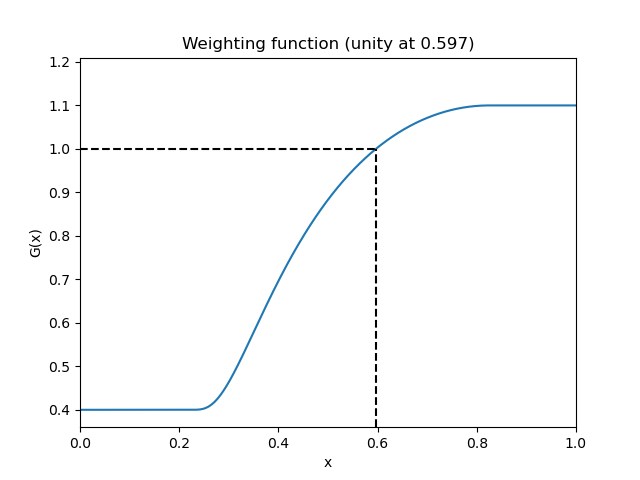
\includegraphics[scale=0.75]{python/plot.png}
  \caption{\label{fig:PlotOfPWF} $\PWF$ plotted over the range $[0,1]$.}
\end{figure}

In light of the definitions in this section, the formula in \eqref{eq:coursework-grade-calculation} can be re-written as
\begin{align*}
  \courseworkGrade = \frac{(\PWF(m_p) \times m_i \times \ipacWeight) + \vivaGrade}{2},
\end{align*}
where the value $(\PWF(m_p) \times m_i \times \ipacWeight)$ is capped at 100\%.